\textbf{Context:} Heterosexual HIV transmission in eSwatini
\hfill\smash{\raisebox{-5.5\baselineskip}{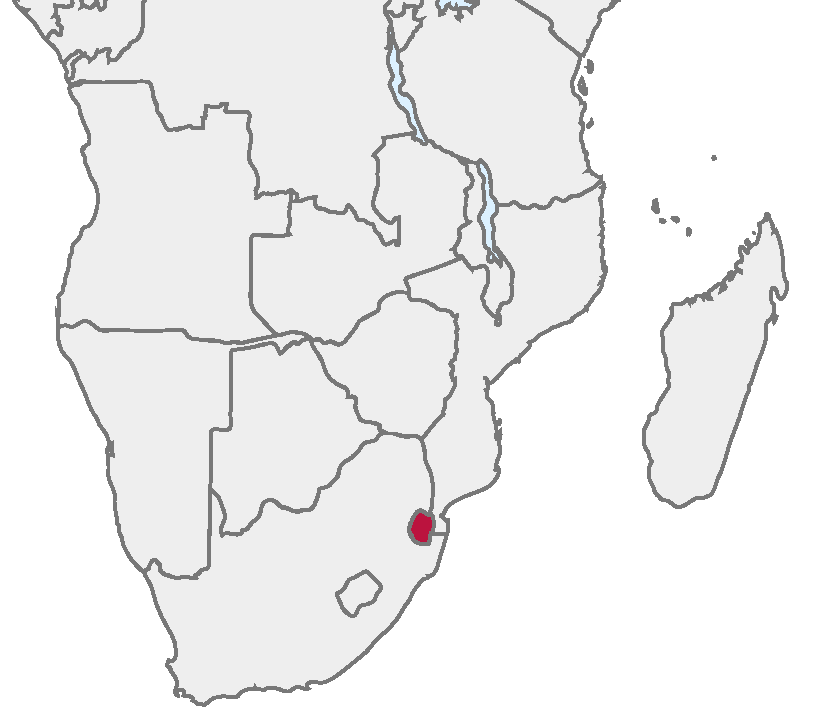
\includegraphics[height=6\baselineskip]{eswatini}\hskip-5mm}}
\paragraph{Full compartmental model:}\unskip
\begin{itemize}
  \item 8 risk groups, 5 HIV stages, 5 treatment cascade states
  \item 4 partnership types, including:\\
        main (12--25 years), casual \& sex work (0--2 years)
  \item Calibrated to HIV prevalence, incidence, treatment cascade data\\
        under \caseinst[black] model; repeat for \caseprop[black] model:
\end{itemize}\bigskip
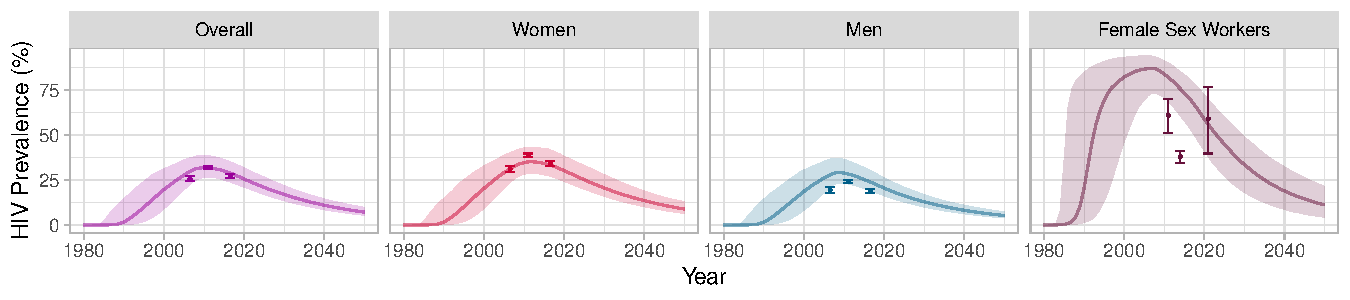
\includegraphics[width=\linewidth]{fit}\unskip\vskip-1ex
\paragraph{Experiment: \textnormal{Compare \caseinst vs \caseprop models:}}
\begin{enumerate}[label=(\alph*),left=0pt]
  \item \textbf{overall incidence}, with equal parameters from \caseprop[black] calibration
        \\$\rightarrow$ direct influence of instantaneous partnerships
  \item \textbf{incidence in longer vs shorter partnerships}, with model-specific parameters
        \\$\rightarrow$ indirect influence on model-inferred prevention priorities
\end{enumerate}
\vskip.2ex
